\documentclass[/home/jesse/Analysis/FemtoAnalysis/AnalysisNotes/AnalysisNoteJBuxton.tex]{subfiles}
\renewcommand{\NonFlatBgdLamKch}{_NonFlatBgdCrctnLamK0LinearLamKchPolynomial}
\renewcommand{\NonFlatBgdLamKs}{_NonFlatBgdCrctnLamK0LinearLamKchPolynomial}

\renewcommand{\ResNum}{_3Res}
\renewcommand{\PrimMaxDecay}{_PrimMaxDecay10fm}

\renewcommand{\SaveNameModLamKch}{\MomRes\NonFlatBgdLamKch\ResNum\PrimMaxDecay\ResMethod\ParamFixAndShareLamKch}
\renewcommand{\SaveNameModLamKs}{\MomRes\NonFlatBgdLamKs\ResNum\PrimMaxDecay\ResMethod\ParamFixAndShareLamKch}

\begin{document}

\subsection{Results: \LamKs and \LamKpm}
\label{ResultsLamK}

In the following sections, we present our final results, for which three residual contributors are assumed.
Results for the cases of ten residual contributors and no residual correlations may be found in Appendices \ref{App_ResultsLamK_10Res} and \ref{App_ResultsLamK_NoRes}, respectively.
Furthermore, comparisons of results obtained using different variations of the fit method can be found in Appendix \ref{App_ResultsLamK_FitMethComp}.

For the results shown, unless otherwise noted, the following hold true:
All correlation functions were normalized in the range 0.32 $< k^{*} <$ 0.40 GeV/c, and fit in the range 0.0 $< k^{*} <$ 0.30 GeV/c.
For the \LamKchM and \ALamKchP analyses, the region 0.19 $< k^{*} <$ 0.23 GeV/$c$ was excluded from the fit to exclude the bump caused by the $\Omega^{-}$ resonance.
The non-femtoscopic backgrounds for the \LamKchP and \LamKchM systems were modeled by a (6$^{\mathrm{th}}$-)order polynomial fit to THERMINATOR simulation, while those for the \LamKs were fit with a simple linear form.
All analyses were fit simultaneously across all centralities, with a single radius and normalization $\lambda$ parameter for each centrality bin.
Scattering parameters ($\Re f_{0}$, $\Im f_{0}$, $d_{0}$) were shared between pair-conjugate systems, but assumed unique between the different \LamK charge combinations (i.e. a parameter set describing the \LamKchP \& \ALamKchM system, a second set describing the \LamKchM \& \ALamKchP system, and a third for the \LamKs \& \ALamKs system).
Each correlation function received a unique normalization parameter.
The fits were corrected for finite momentum resolution effects, non-femtoscopic backgrounds, and residual correlations resulting from the feed-down from resonances.

Lines and boxes on the experimental data represent statistical and systematic errors, respectively.
In the figures showing experimental correlation functions with fits, the black solid curve represents the primary (\LamK) correlation's contribution to the fit.
The green line shows the fit to the non-flat background.  
The purple points show the fit after all residual contributions have been included, and momentum resolution and non-flat background corrections have been applied.
The extracted fit values with uncertainties are printed as (fit value) $\pm$ (statistical uncertainty) $\pm$ (systematic uncertainty).


Figure \ref{fig:ScattParams_3Res} nicely collects and summarizes all of our extracted fit parameters.
In the summary plot, we show the extracted scattering parameters in the form of a $\Im f_{0}$ vs $\Re f_{0}$ plot, which includes the $d_{0}$ values to the right side.  
We also show the $\lambda$ vs. radius parameters for all three of our studied centrality bins.  
The extracted fit parameters are also collected in Table \ref{tab:FitResultsLamK_3Res}.
Figure \ref{fig:mTScalingOfRadii_3Res} presents our extracted fit radii, along with those of other systems previously analyzed by ALICE \cite{Adam:2015vja}, as a function of pair transverse mass (\mt).

%%%%%%%%%%%%%%%%%%%%%%%%%%%%%%%%%%%%%%%%     TABLES!!!!!     %%%%%%%%%%%%%%%%%%%%%%%%%%%%%%%%%%%%%%%%
\begin{comment}
\begin{landscape}
\subfile{\ResultsDirBaseLamKch\SaveNameModLamKch/Tables/ResultsTableTriple.tex}
\end{landscape}
\end{comment}

%%\label{tab:FitResultsLamK_3Res}
\subfile{\ResultsDirBaseLamKch\SaveNameModLamKch/Tables/ResultsTableTriple_Vert.tex}

%%%%%%%%%%%%%%%%%%%%%%%%%%%%%%%%%%%%%%%%%%%%%%%%%%%%%%%%%%%%%%%%%%%%%%%%%%%%%%%%%%%%%%%%%%%%%%%%%%%%%

\begin{figure}[h]
  \centering
  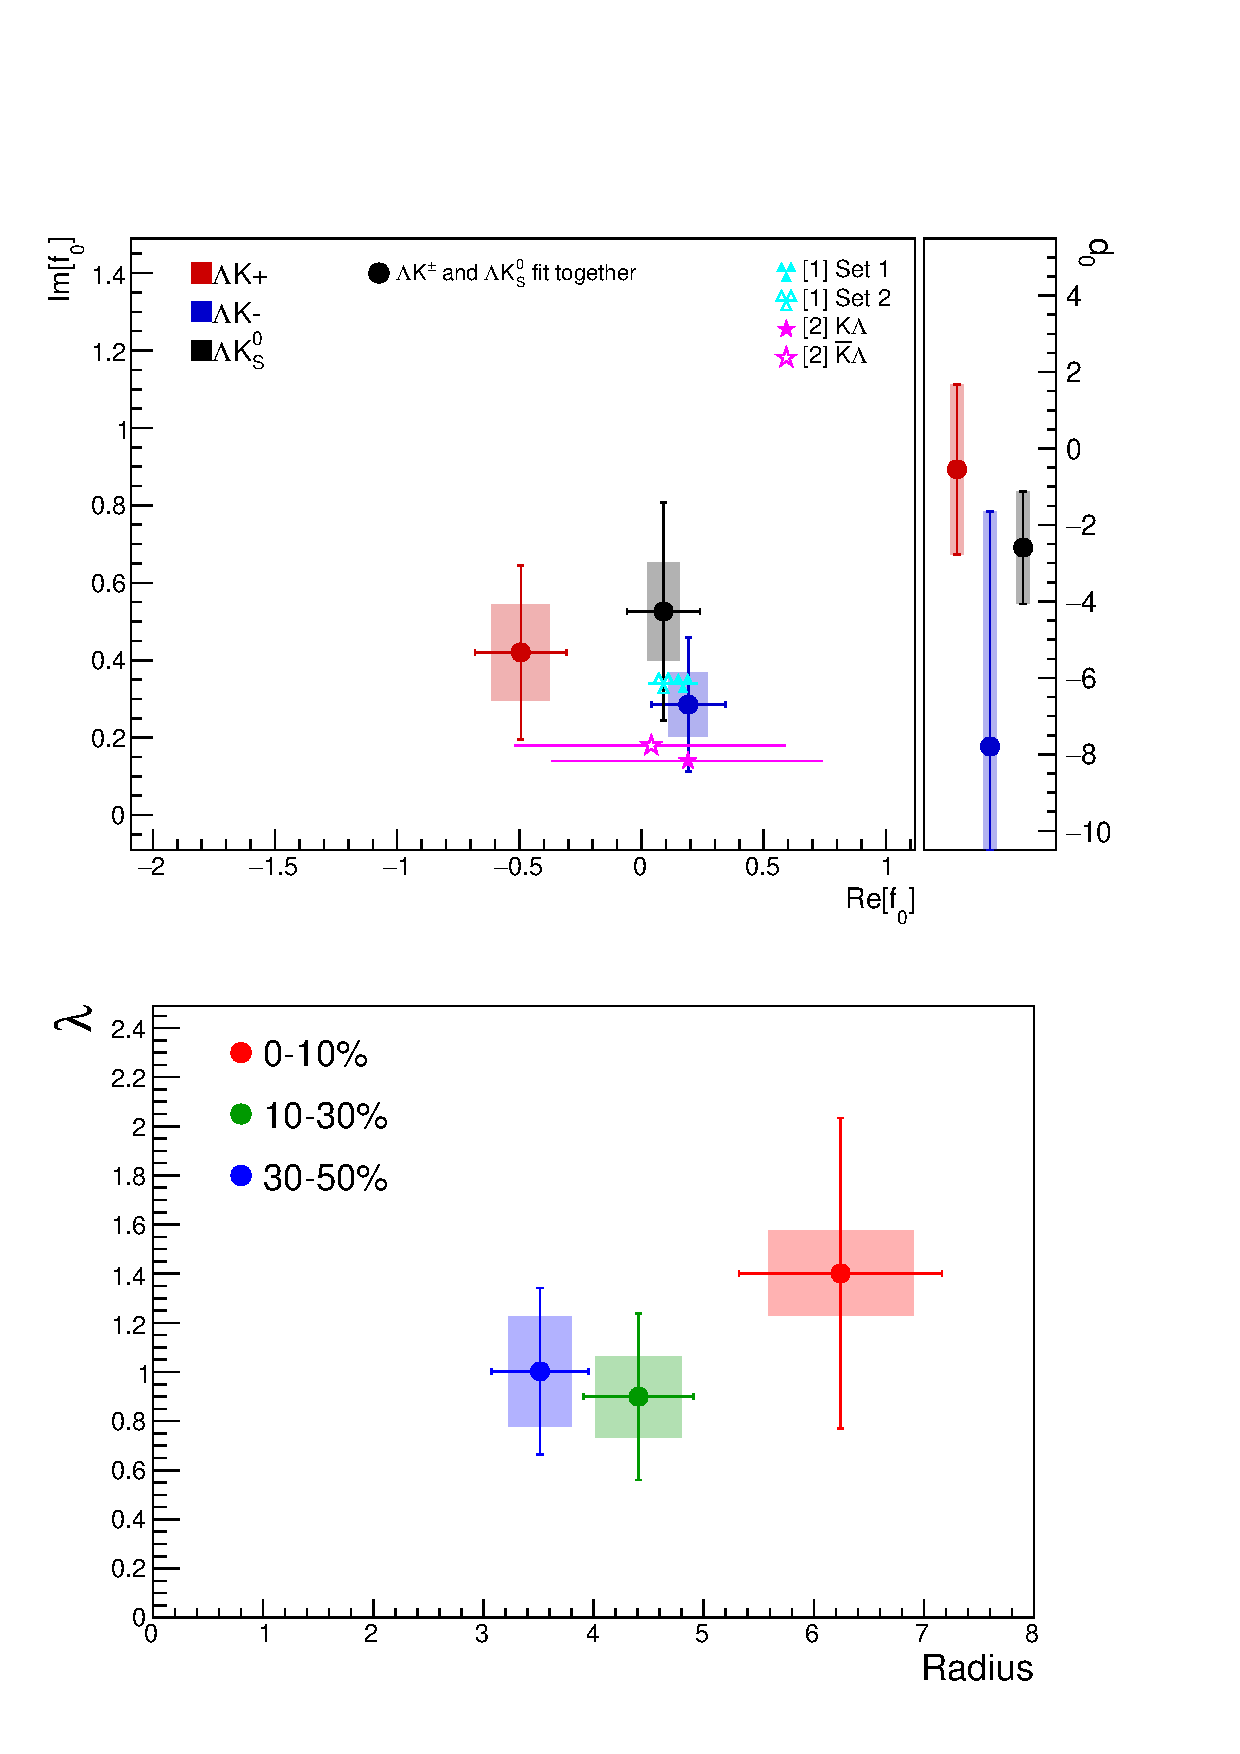
\includegraphics[width=0.85\textwidth]{\ResultsDirBaseLamKch\SaveNameModLamKch/Comparisons/FinalResults_Comp3An_Vertical.pdf}
  \caption[Extracted scattering parameters]
  {
  Extracted fit parameters for the case of 3 residual contributors for all of our \LamK systems.  
  [Top]: $\Im f_{0}$ vs. $\Re f_{0}$, together with $d_{0}$ to the right.  
  [Bottom]: $\lambda$ vs. Radius for the 0-10\% (blue), 10-30\% (green), and 30-50\% (red) centrality bins.  
  In the fit, all \LamK systems share common radii.
  The color scheme used in the panel are to be consistent with those in Fig. \ref{fig:mTScalingOfRadii_3Res}.
  The cyan ([A] = Ref. \cite{Liu:2006xja}) and magenta ([B] = Ref. \cite{Mai:2009ce}) points show theoretical predictions made using chiral perturbation theory.
  }
  \label{fig:ScattParams_3Res}
\end{figure}

\begin{figure}[h]
  \centering
  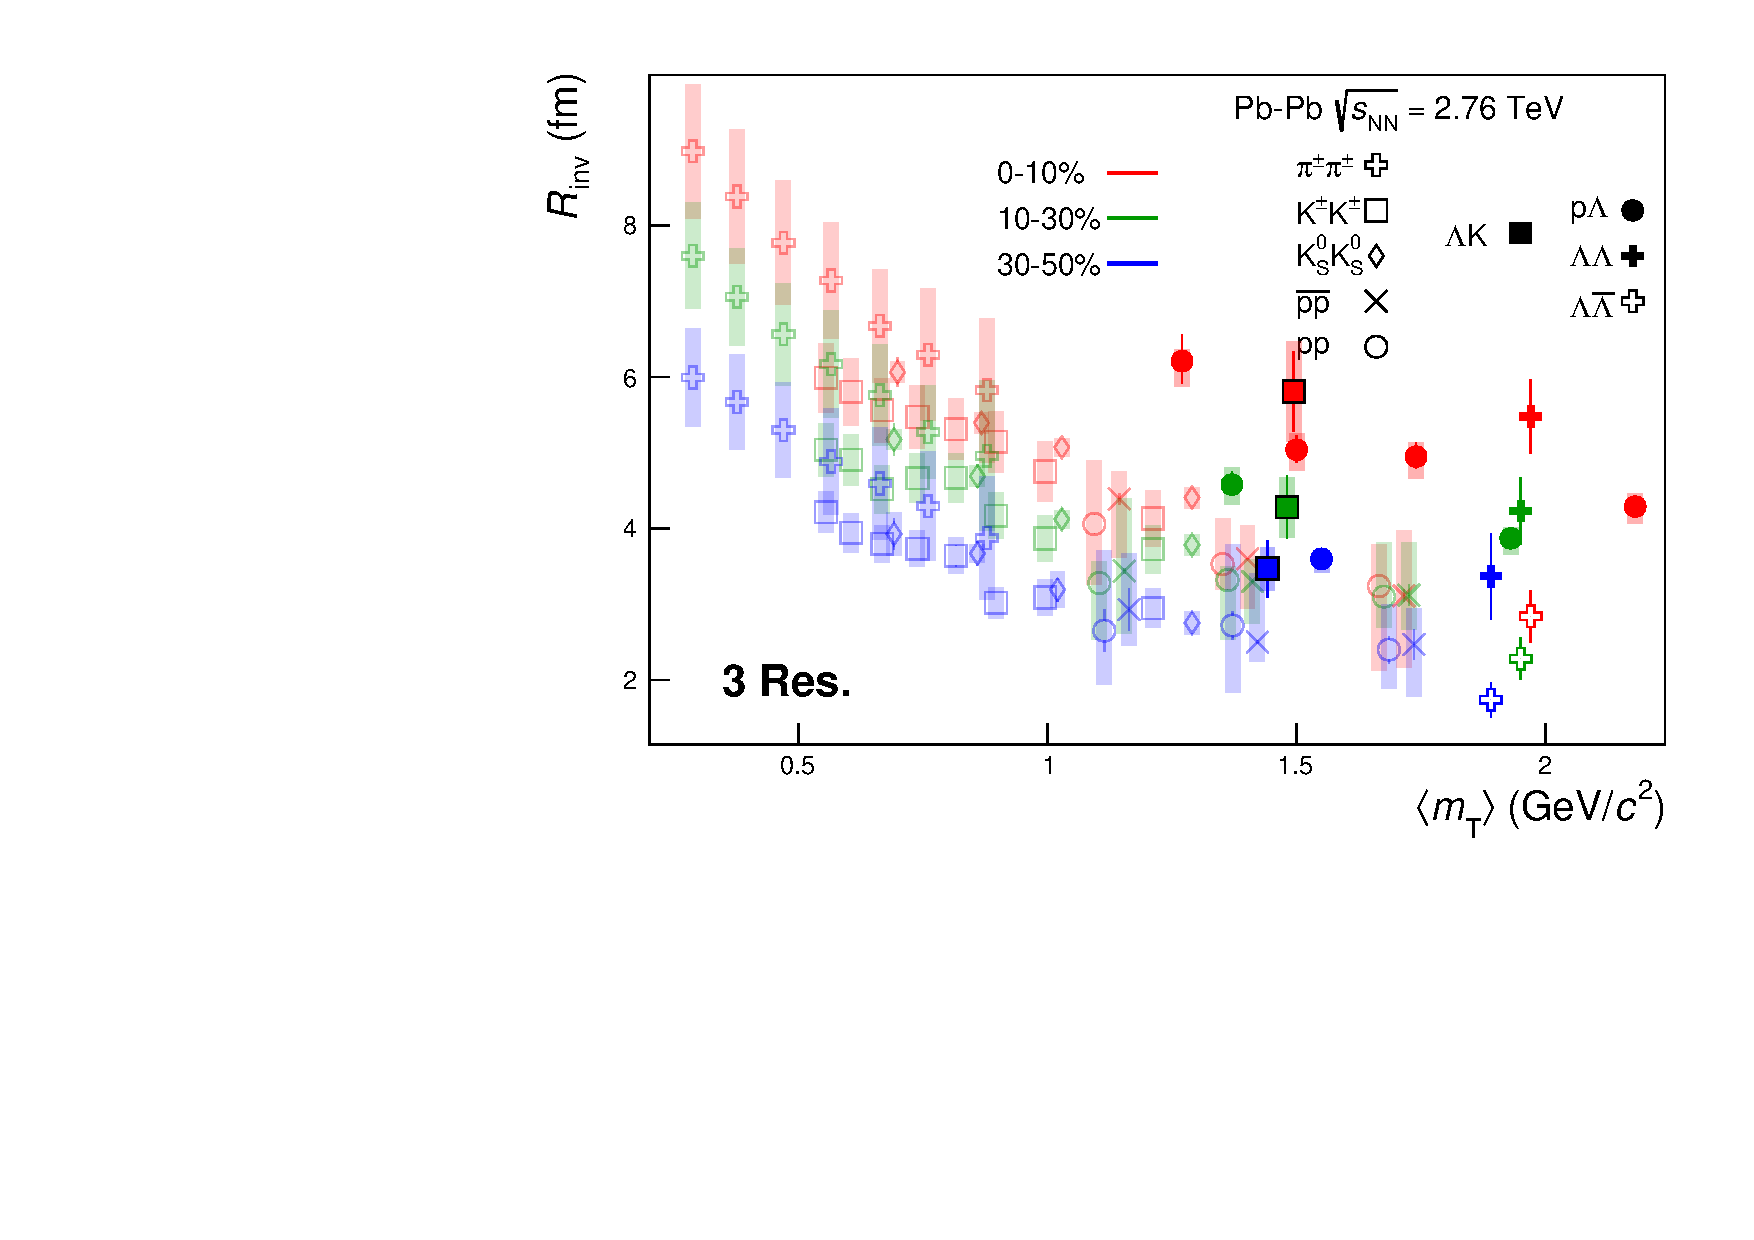
\includegraphics[width=\textwidth]{\ResultsDirBaseLamKch\SaveNameModLamKch/Comparisons/mTscaling_MinvCalc_OutlinedPoints_OthersTransparent_wJaiAndHans_3Res.pdf}
  \caption[$m_{\mathrm{T}}$ scaling of radii]
  {
  3 residual correlations in \LamK fits.  
  Extracted fit $R_{\mathrm{inv}}$ parameters as a function of pair transverse mass ($m_{\mathrm{T}}$) for various pair systems over several centralities. 
  The ALICE published data \cite{Adam:2015vja} are shown with transparent, open symbols.  
  The new \LamK results are shown with opaque, filled symbols.  
  The \mt value for the \LamK system is an average of those for the \LamKchP, \ALamKchM, and \LamKs systems.
  }
  \label{fig:mTScalingOfRadii_3Res}
\end{figure}


\clearpage

\subfile{7_ResultsAndDiscussion/7.1_ResultsLamK/7.1.1_ResultsLamK_CorrFctnsWFits/7.1.1_ResultsLamK_CorrFctnsWFits.tex}
\subfile{7_ResultsAndDiscussion/7.1_ResultsLamK/7.1.2_ResultsLamK_DiscussionOfmTScaling/7.1.2_ResultsLamK_DiscussionOfmTScaling.tex}

\end{document}